\documentclass[12pt,a4paper]{article}

\usepackage[utf8]{inputenc}
\usepackage[T1]{fontenc}
\usepackage{amsmath}
\usepackage{geometry}
\usepackage{booktabs}
\usepackage{graphicx}
\usepackage{xcolor}
\usepackage{float}

\geometry{margin=1in}

\title{Report 3: Logistic Regression}
\author{Dao Quy Tung - 2540101}
\date{May 13, 2026}

\begin{document}

\maketitle

\section{Introduction}

The objective of this labwork is to implement logistic regression from scratch using gradient descent.
The model is trained on a loan decision dataset, where each profile has two input features: salary and experience.
The output label is binary:

\[
y = 1 \text{ for loan}, \quad y = 0 \text{ for refuse}
\]

This labwork contains two parts. The first part implements logistic regression with binary cross entropy loss. The extra part computes the same loss using the expression derived from the sigmoid formulation:

\[
L_i = -y_i z_i + \log(1 + e^{z_i})
\]

The dataset used in the experiment is:

\begin{table}[H]
\centering
\begin{tabular}{ccc}
\toprule
Experience & Salary & Loan \\
\midrule
3.00 & 4 & 1 \\
2.50 & 4 & 1 \\
1.00 & 4 & 0 \\
2.50 & 5 & 1 \\
2.00 & 5 & 1 \\
1.50 & 5 & 0 \\
0.50 & 5 & 0 \\
1.75 & 6 & 1 \\
0.25 & 6 & 0 \\
1.00 & 7 & 1 \\
0.25 & 7 & 0 \\
0.20 & 7 & 0 \\
0.15 & 7 & 0 \\
2.00 & 8 & 1 \\
1.00 & 8 & 0 \\
0.15 & 8 & 0 \\
0.10 & 8 & 0 \\
0.50 & 9 & 1 \\
1.00 & 10 & 1 \\
\bottomrule
\end{tabular}
\caption{Training data from \texttt{loan2.csv}.}
\end{table}

\section{Logistic Regression Algorithm}

The logistic regression model first computes a linear score:

\[
z = w_1x_1 + w_2x_2 + w_0
\]

In this experiment:

\[
x_1 = salary, \quad x_2 = experience
\]

The score \(z\) is converted into a probability using the sigmoid function:

\[
\hat{y} = \sigma(z) = \frac{1}{1 + e^{-z}}
\]

The predicted value \(\hat{y}\) is interpreted as the estimated probability that the profile belongs to class \(1\), which means loan.

For the basic experiment, the loss is binary cross entropy:

\[
L_i = -(y_i\log(\hat{y}_i) + (1-y_i)\log(1-\hat{y}_i))
\]

For the extra experiment, the same loss is computed using:

\[
L_i = -y_i z_i + \log(1 + e^{z_i})
\]

The parameters are updated using gradient descent. For each data point, the error term is:

\[
e_i = \hat{y}_i - y_i
\]

The gradients are accumulated as:

\[
\frac{\partial L_i}{\partial w_0} = e_i
\]

\[
\frac{\partial L_i}{\partial w_1} = e_i x_1
\]

\[
\frac{\partial L_i}{\partial w_2} = e_i x_2
\]

\section{Implementation}

The implementation reads the training data from \texttt{loan2.csv}. The input features are stored as salary and experience, and the target label is stored as the loan decision.

The main steps are:

\begin{enumerate}
  \item Read the training data from the CSV file.
  \item Initialize \(w_0\), \(w_1\), and \(w_2\).
  \item Compute \(z = w_1x_1 + w_2x_2 + w_0\).
  \item Compute the probability \(\hat{y} = \sigma(z)\).
  \item Compute the loss.
  \item Compute the gradients from \(\hat{y}-y\).
  \item Update the weights using the learning rate.
  \item Repeat for the selected number of epochs.
\end{enumerate}

Two versions were tested:

\begin{table}[H]
\centering
\begin{tabular}{lcc}
\toprule
Version & Initial parameters & Reported loss \\
\midrule
Basic logistic regression & \(w_0=0, w_1=1, w_2=2\) & Binary cross entropy \\
Logistic regression extras & \(w_0=0, w_1=1, w_2=2\) & \(-yz + \log(1+e^z)\) \\
\bottomrule
\end{tabular}
\caption{Two implementations used in Labwork 3.}
\end{table}

\section{Experiment Output and Learning Rate Analysis}

The basic experiment was executed with:

\[
w_0 = 0, \quad w_1 = 1, \quad w_2 = 2, \quad r = 0.1
\]

The number of epochs was set to \(190000\). The test profile was:

\[
salary = 7.0, \quad experience = 0.5
\]

Selected output from the basic experiment:

\begin{table}[H]
\centering
\begin{tabular}{rrrrr}
\toprule
Epoch & Loss & \(w_0\) & \(w_1\) & \(w_2\) \\
\midrule
0 & 2.7576 & -0.053 & 0.658 & 1.973 \\
10000 & 0.2102 & -12.406 & 1.152 & 4.258 \\
50000 & 0.1985 & -17.867 & 1.721 & 5.619 \\
100000 & 0.1983 & -18.688 & 1.805 & 5.831 \\
150000 & 0.1983 & -18.797 & 1.816 & 5.859 \\
189999 & 0.1983 & -18.811 & 1.818 & 5.863 \\
\bottomrule
\end{tabular}
\caption{Selected output of the basic logistic regression experiment.}
\end{table}

The final parameters are:

\[
w_0 = -18.811, \quad w_1 = 1.818, \quad w_2 = 5.863
\]

For the test profile, the predicted probability is:

\[
\hat{y} = 0.0409
\]

With threshold \(0.5\), the final decision is:

\[
\text{REFUSE}
\]

\begin{figure}[H]
\centering
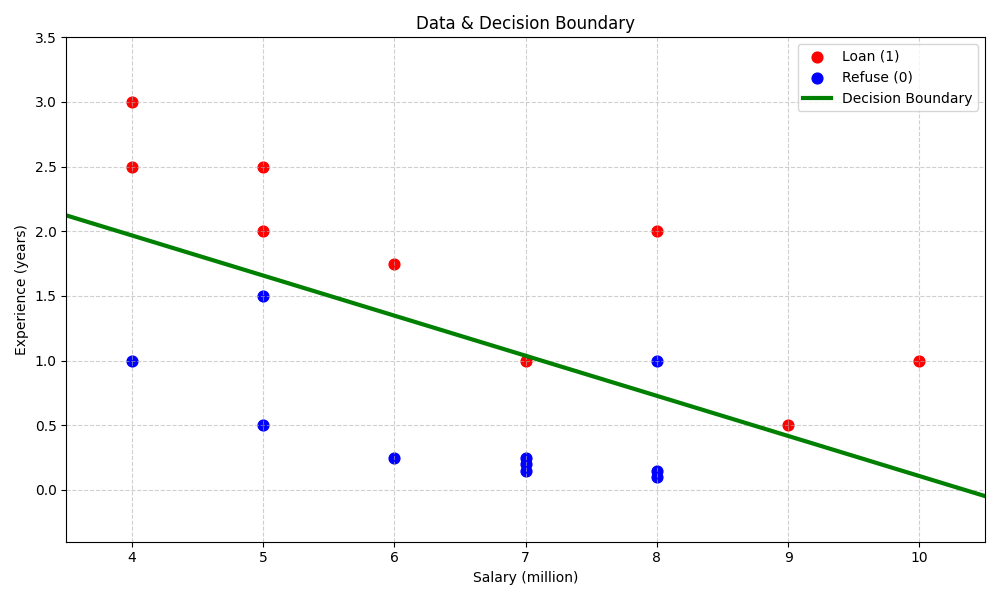
\includegraphics[width=0.85\textwidth]{logistic_regression_result.png}
\caption{Linear regression result for the extra experiment.}
\end{figure}


The extra experiment was executed with the same initial parameters, learning rate, epochs, and test profile.
Selected output from the extra experiment:

\begin{table}[H]
\centering
\begin{tabular}{rrrrr}
\toprule
Epoch & Loss & \(w_0\) & \(w_1\) & \(w_2\) \\
\midrule
0 & 2.7576 & -0.053 & 0.658 & 1.973 \\
10000 & 0.2102 & -12.406 & 1.152 & 4.258 \\
50000 & 0.1985 & -17.867 & 1.721 & 5.619 \\
100000 & 0.1983 & -18.688 & 1.805 & 5.831 \\
150000 & 0.1983 & -18.797 & 1.816 & 5.859 \\
189999 & 0.1983 & -18.811 & 1.818 & 5.863 \\
\bottomrule
\end{tabular}
\caption{Selected output of the logistic regression extra experiment.}
\end{table}

The final prediction of the extra experiment is also:

\[
\hat{y} = 0.0409
\]

Therefore, the final decision is also:

\[
\text{REFUSE}
\]

Both experiments produce the same output because they use the same model and the same gradient update. The difference is only in how the loss value is computed.

\begin{figure}[H]
\centering
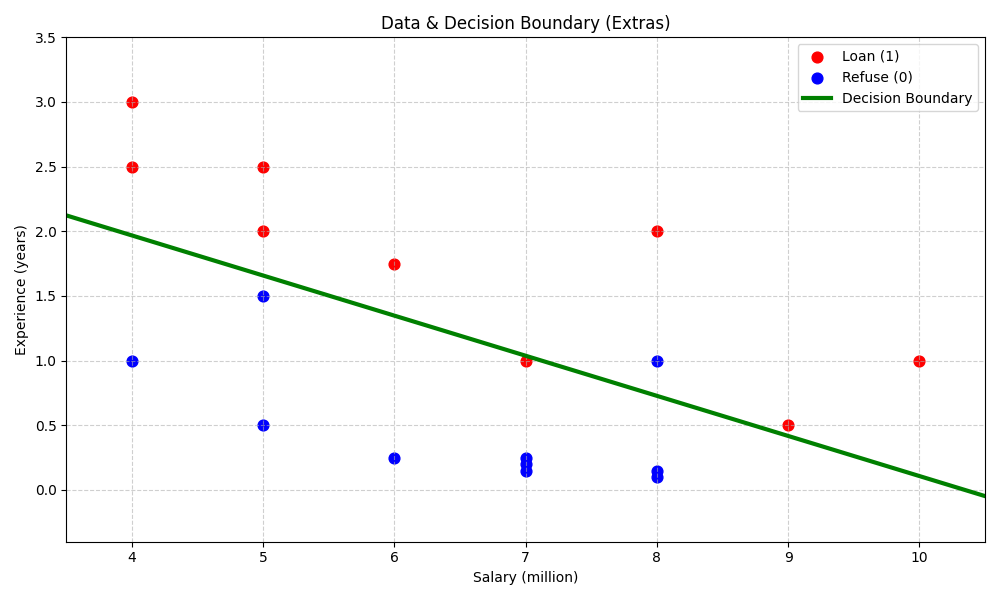
\includegraphics[width=0.85\textwidth]{logistic_regression_extra_result.png}
\caption{Linear regression result for the extra experiment.}
\end{figure}

\subsection{Learning Rate Comparison}

Different learning rates were tested with the same initial parameters and \(190000\) epochs:

\begin{table}[H]
\centering
\begin{tabular}{lrrrrr}
\toprule
Learning rate & Loss & \(w_0\) & \(w_1\) & \(w_2\) & Decision \\
\midrule
0.01 & 0.2020 & -14.978 & 1.423 & 4.888 & REFUSE \\
0.05 & 0.1983 & -18.660 & 1.802 & 5.824 & REFUSE \\
0.10 & 0.1983 & -18.811 & 1.818 & 5.863 & REFUSE \\
0.20 & 0.1983 & -18.814 & 1.818 & 5.864 & REFUSE \\
0.50 & 0.1983 & -18.814 & 1.818 & 5.864 & REFUSE \\
\bottomrule
\end{tabular}
\caption{Effect of different learning rates.}
\end{table}

With a small learning rate such as \(0.01\), the loss is still slightly higher after \(190000\) epochs. The learning rates \(0.05\), \(0.1\), \(0.2\), and \(0.5\) reach almost the same loss value, around \(0.1983\).

However, a larger learning rate is not always safer. A very large value may make gradient descent unstable on other datasets or with different settings. In this experiment, all tested learning rates still lead to the same final decision for the test profile.

\section{Conclusion}

In this labwork, logistic regression was implemented from scratch using gradient descent.
Both the basic experiment and the extra experiment reached almost the same final parameters:

\[
w_0 = -18.811, \quad w_1 = 1.818, \quad w_2 = 5.863
\]

For the test profile with salary \(7.0\) and experience \(0.5\), the predicted probability is \(0.0409\). Since this value is smaller than the threshold \(0.5\), the final decision is \(\text{REFUSE}\).

The experiments show that logistic regression can be used to model a binary decision problem. The learning rate affects how fast the loss decreases during training, and choosing a suitable learning rate is important for stable convergence.

\end{document}
